\documentclass[11pt]{article}
\usepackage[a4paper, margin=1.5cm]{geometry}
\usepackage[utf8]{inputenc}
\usepackage{babel}
\usepackage[spanish]{layout}
\usepackage[article]{ragged2e}
\usepackage{textcomp}
\usepackage{amsmath}
\usepackage{amssymb}
\usepackage{amsfonts}
\usepackage{proof}
\usepackage{enumerate}
\usepackage{graphicx}
\usepackage{multirow}

\setlength{\parindent}{0pt}

\title{
    Ontología del Mundo Mágico de Harry Potter}
\author{Mellino, Natalia \and Farizano, Juan Ignacio}
\date{}

\begin{document}
\maketitle

\noindent\rule{\textwidth}{1pt}

\section{Descripción}

\-\ Nos interesa estudiar las diferentes escuelas del mundo mágico de Harry Potter.
Cada escuela puede estar divida en 4 casas o en ninguna, donde los alumnos serán 
repartidas en ellas. Cada casa tiene un jefe y dos prefectos, un hombre y una 
mujer. Un jefe es siempre un profesor de la escuela, mientras que los roles de 
prefectos los ocupan dos estudiantes de esa misma casa que estén cursando desde 
quinto año en adelante.

\-\ Los personajes en este mundo mágico las podemos categorizar según el nivel de 
magia que posean: Magos o Brujas, Squibs o Muggles. Los Magos o Brujas son 
aquellos que poseen magia, los Squibs son los que no tienen magia pero provienen 
de padres magos mientras que los Muggles no poseen nada de magia. En este mundo, 
sólo los Magos o Brujas pueden ser alumnos o profesores de una escuela.

\-\ En una escuela los estudiantes deben atender a clases que se dictan durante todo 
el año. Las clases van variando a medida que van avanzando de año. Un alumno se 
gradua al finalizar séptimo año.
Durante el año, los alumnos tiene diferentes actividades recreativas, siendo las 
más importantes:
    \begin{itemize}
        \item La Copa de las Casas que es un galardón otorgado al final de cada 
        año a la casa que reunió más puntos durante el transcurso del año 
        mediante diferentes actividades.
        \item La principal disciplina es el famoso deporte mágico Quidditch, 
        cada casa tiene su propio equipo, el cual esta conformado por siete 
        jugadores y tiene un capitán que puede ser cualquiera de los integrantes 
        del equipo. En este deporte, compiten en un campeonato las casas de las 
        escuelas entre sí. 
    \end{itemize}

\textbf{Observación:} el razonador elegido para probar la ontología es \emph{Pellet}.
    
\newpage

\section{Modelado de la ontología}

\begin{figure}[h!]
    \begin{center}
      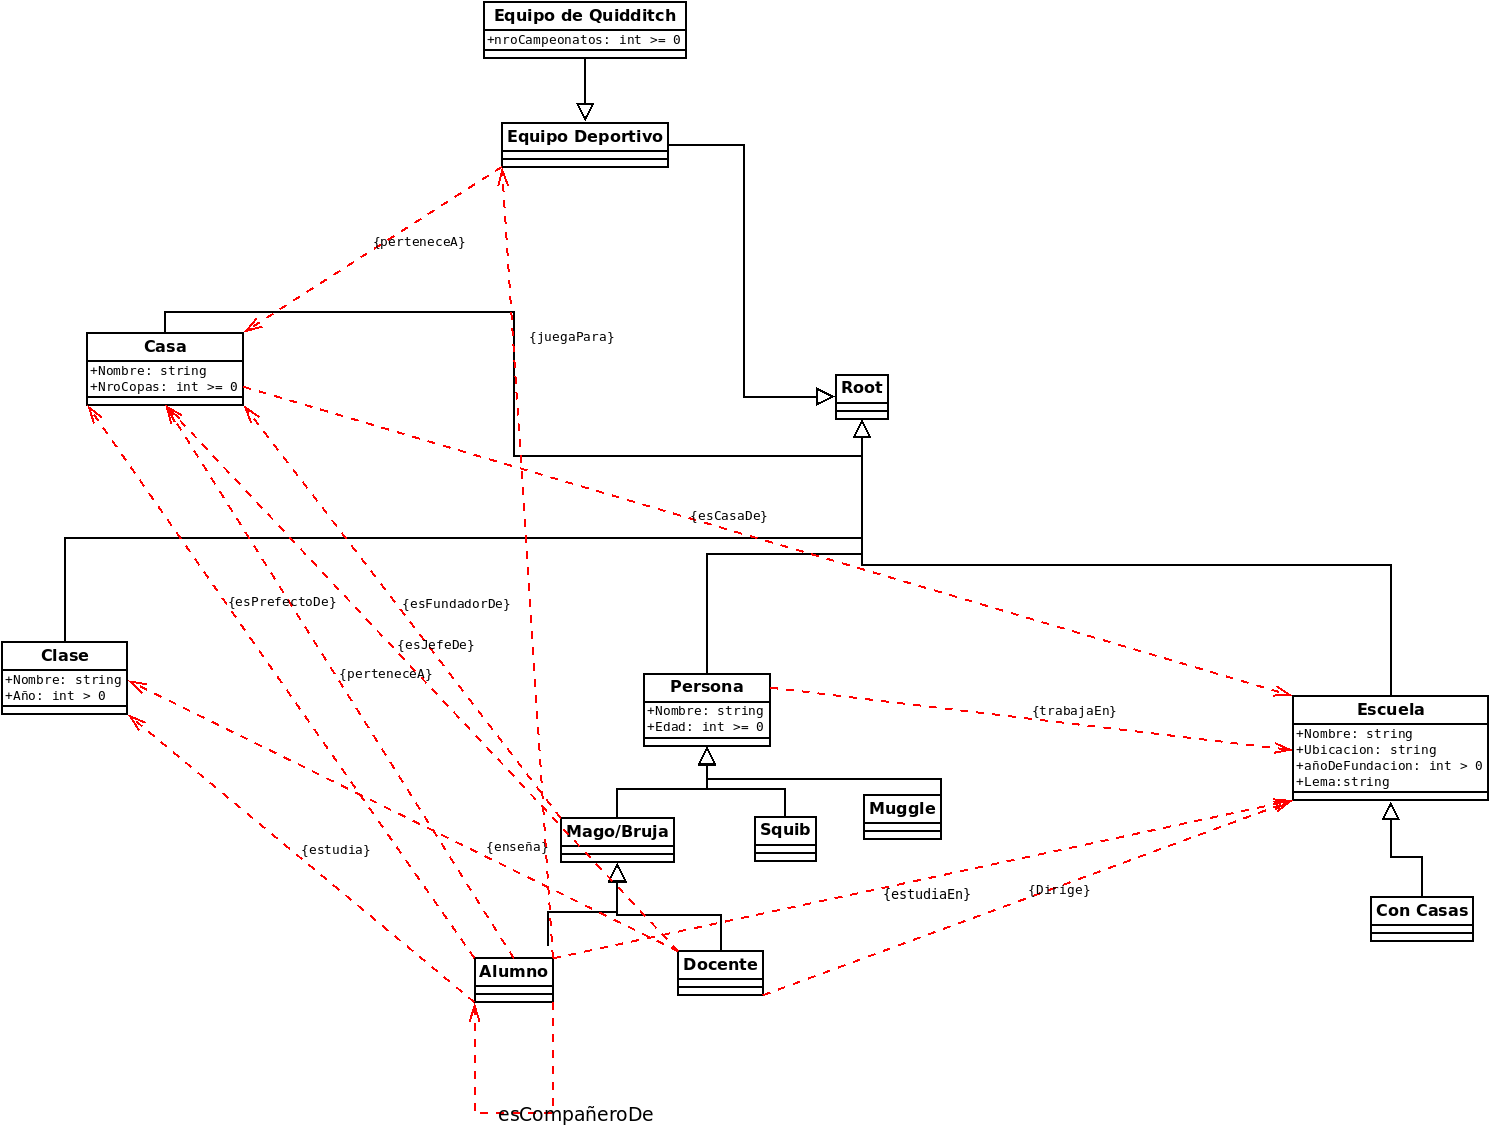
\includegraphics[width=\linewidth]{harrypotter.png}
    \end{center}
  \end{figure}

En rojo se pueden ver las distintas relaciones entre las clases. En Protégé se 
han realizado también las \textbf{relaciones inversas} para la mayoría de las 
relaciones presentadas.

\section{Queries}

Las queries elegidas para probar nuestra ontología fueron las siguientes:

\begin{itemize}
    \item \texttt{Casa and lePertenece some (EquipoDeQuidditch and CampeonatosGanados value 5)}
    \item \texttt{Alumno and estudia value Pociones and perteneceA value Gryffindor}
\end{itemize}

\section{Conclusiones}

\begin{itemize}
    \item En general no se presentaron dificultades con el modelado de las clases
          y las relaciones, ya que el tópico de la ontología nos resulta bastante
          familiar y es de nuestro agrado.
    \item Nuestra mayor dificultad se nos presentó al momento de querer componer
          relaciones, por ejemplo si un alumno pertence a una casa determinada 
          entonces nosotros podemos deducir que ese alumno estudia en la escuela 
          de esa casa. Pero el razonador no podía inferir eso sin tener la
          composición de las relaciones \emph{perteneceA} y \emph{esCasaDe}. 
          Finalmente, pudimos lograr resolver el inconveniente y lograr el 
          resultado deseado.
    \item Una cosa que no pudimos resolver es hacer que el razonador infiera que
          si un alumno \emph{juegaPara} el Equipo Deportivo de una Casa, entonces
          el alumno \emph{perteneceA} esa casa. 
\end{itemize}

\end{document}